\documentclass{beamer}
\renewcommand\thesection{\arabic{section}}
\newcommand{\myfont}{\rmfamily\normalsize\upshape\mdseries}
\newcommand{\degree}{^\circ}
\title{\sffamily Part 0-Math Foundation}  
\institute[UM-SJTU JI]{University of Michigan-Shanghai Jiao Tong University Joint Institute}
\author{HamHam}
\usepackage{graphicx}
\usepackage{picinpar}
\usepackage{indentfirst}
\usepackage{chemformula}
\usepackage{geometry}
\usepackage{subfigure}
\usepackage{appendix}
\usepackage{amsfonts,amsmath,amssymb}
\usepackage{enumerate}
\usepackage{float}
\usepackage{geometry}
\usepackage{latexsym}
\usepackage{listings}
\usepackage{multicol,multirow,multido}
\usepackage{tabularx}
\usepackage{ulem}
\usepackage{tikz}
\usepackage{xcolor}
\usepackage{cite}
\usepackage{setspace}
\usepackage{hyperref}
\usepackage{textpos}
\usepackage{booktabs}

\usetheme[dove]{Boadilla}
\usecolortheme{dolphin}
\useoutertheme{miniframes}
\begin{document}
    \usebackgroundtemplate{\tikz\node[opacity=0.3]{
    
\includegraphics[width=\paperwidth,
    height=\paperheight]{hamster.jpg}
    };}
\begin{titlepage}
    \begin{center}
        VV186 - Honors Mathmatics II
    \end{center}
\end{titlepage}
\myfont

\begin{frame}
    \frametitle{About Exam}
    \begin{itemize}
        \item 30 pts, possibly contain
        \begin{itemize}
            \item[1.] Multiple choice questions (The choices can be all wrong.)
            \item[2.] Calculation question
            \item[3.] Proof question 
            \item[4.] Explanation question 
            \item[5.] ...
        \end{itemize}
        \item 100 mins (8:00 - 9:40). \textcolor{red}{Do Wake Up!}
        \item 100/30 = 3.3 mins/pt. Therefore, you probably don’t want to spend more
        than 5 mins on 1 pt.
        \item Don’t panic if you cannot figure out all some specific question. Just skip it
        and do it later.
        \item The questions may not be arranged in the order of difficulty.
    \end{itemize}
\end{frame}
\begin{frame}
    \frametitle{Checking List}
    \begin{itemize}
        \item Statement/Truth Table
        \item Prove by Contraposition
        \item Logical/Sets Operation
        \item Cartesian product/ Ordered pairs
        \item Properties of Natural/Rational/Complex Numbers
        \item Concept of Interval/Points/Sets
        \item \textbf{Mathematical Induction}
    \end{itemize}
    \vspace{1em}\hspace{1em}
    Part 0 is \textbf{not} the key point of the exam. However, you should still go through
these concepts. Though they might not be directly tested, they could occur
somewhere in your exam paper.
\end{frame}
\begin{frame}
    \frametitle{Truth Table}
    \begin{figure}
        \centering
        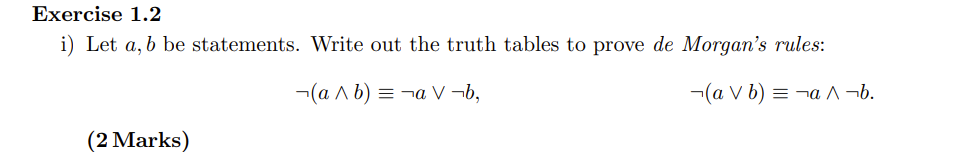
\includegraphics[width=0.9\textwidth]{ex1.png}
    \end{figure}
    \hspace{1em}
        Notice that the last column of the truth table should be an evaluation on equivalence. 
    For example, for the first question, you should evaluate $\neg (a \wedge b)\Leftrightarrow \neg a \vee \neg b$. 
    It is supposed to be true for the whole column. 
    Only through this fact can you conclude that 
    $\neg(a \wedge b) \equiv \neg a\vee \neg b$.
    \\ \hspace{1em}
    Please distinguish equivalence ($\Leftrightarrow$) and logical equivalence ($\equiv$). 
    The former one is a binary operation, 
    while the later one indicates a relationship 
    between two compound statements. To be more precise, logical equivalence indicates that the equivalence between two compound statements is a tautology.
\end{frame}
\begin{frame}
    \frametitle{Contraposition}
    The famous \textbf{tautology}
    $$(A \Rightarrow B) \equiv (\neg B \Rightarrow \neg A)$$
is useful in some situation. If you are asked to prove some statement $A \Rightarrow B$ but
you cannot find a simple way, you can try to prove by contraposition.
    \vspace{2em}
\end{frame}
\begin{frame}
    \frametitle{Exercise}
    Let $x \in \mathbb{Z}$. If $x^2-6x+5$ is even, then $x$ is odd.\\
    \pause
    \vspace{2em}
    \textbf{Proof:} Suppose that $x$ is even. Then we want to show that $x^2 - 6x + 5$ is odd.
    Write $x = 2a$ for some $a \in \mathbb{Z}$, and plug in:
    \begin{align*}
        x^2-6x+5 &= (2a)^2-6 (2a)+5 \\
                 &= 4 a^2 -12 a +5 \\
                 &= 2 (2a^2-6a +2)+1 
    \end{align*}
    Thus $x^2-6x+5$ is odd.
\end{frame}
\begin{frame}
    \frametitle{Mathematical Induction}
    \hspace{1em}Often one wants to show that some statement frame $A(n)$ is true for 
    all $n \in \mathbb{N}$ with $n\geq n_0 $ for some $n_0\in \mathbb{N}$. 
    Mathematical induction works by establishing two statements:
    \begin{itemize}
        \item[(I)] $A(n_0)$ is true.
        \item[(II)] $A(n+1)$ is true whenever $A(n)$ is true for $n\geq n_0$, i.e.,
        $$\underset{n\geq n_0}{\underset{n\in \mathbb{N}}{\forall}} A(n)\Rightarrow A(n+1)$$ 
    \end{itemize}
    \textbf{Remark:} Mathematical Induction is basically the only relatively important
    concept in Part 0 of VV186. Please see Ex5, Ex6 and Ex7 in sample exam and see
    the related rubric.
    

\end{frame}
\begin{frame}
    \frametitle{Exercise}
    Let $ a_n$ be the following expression with $n$ nested radicals:\
    $$a_n=\sqrt{2+\sqrt{2+\cdots+\sqrt{2+\sqrt{2}}}}$$
    Prove that $a_n = 2 \cos \frac{\pi}{2^{n+1}}$
\end{frame}
\begin{frame}
    \frametitle{Exercise}
    \textbf{Proof:} Note that $a_n$ can be defined recursively like this: $a_1 =\sqrt{2}$, and
    $a_{n+1} =\sqrt{a_n+2}$ for $n \geq 1$. We proceed by induction. For $n = 1$ we have in fact
    $a_1=\sqrt{2}$, and $2\cdot \cos \frac{\pi}{4}= 2\cdot \frac{1}{\sqrt{2}}=\sqrt{2}$.\\ 
    \vspace{1em}
    Next, assuming the result is true for some $n \geq 1$, we have
    \begin{align*}
        a_{n+1}&=\sqrt{2+a_n}=\sqrt{2+2\cos \frac{\pi}{2^{n+1}}}\\
               &=\sqrt{2+2\cos 2\frac{\pi}{2^{n+1}}}\\
               &=\sqrt{2+2(2\cos^2\frac{\pi}{2^{n+2}}-1)}\\
               &=\sqrt{4\cos ^2\frac{\pi}{2^{n+2}}}
               =2\cos \frac{\pi}{2^{n+2}}
    \end{align*}
    By  induction, we conclude that $a_n = 2 \cos \frac{\pi}{2^{n+1}}$.
\end{frame}
\begin{frame}
    \frametitle{Complex Numbers}
    \hspace{1em}
    Given $z_1=(a_1,b_1)$ and $z_2=(a_2,b_2)$
\begin{itemize}
    \item $z_1+z_2=(a_1,b_1)+(a_2,b_2)=(a_1+a_2,b_1,b_2)$
    \item $z_1\cdot z_2=(a_1,b_1)\cdot (a_2,b_2)=(a_1a_2-b_1b_2,a_1b_2-a_2b_1)$
    \item $c\cdot z_1=c(a_1,b_2)=(ca_1,cb_1), c\in \mathbb{R} $
    \item $\bar{z_1}=(a_1,-b_1)$
    \item $|z_1|^2=a_1^2+b_1^2=z_1\bar{z_1}$
    \item Re $z_1= \frac{z_1+\bar{z_1}}{2}$
    \item $($Im $z_1 )i= \frac{z_1-\bar{z_1}}{2}$
    \item $2(|z_1|^2+|z_2|^2)=|z_1+z_2|^2+|z_1-z_2|^2$
    \item $|z_1+z_2|\leq |z_1|+|z_2|$ \textbf{(Triangle Inequality)}
\end{itemize}
\textcolor{red}{Note that the ordering relation is not defined in $\mathbb{C}$!}
\end{frame}
\begin{frame}
    \frametitle{Concept of Interval/Points/Sets}
    \begin{itemize}
        \item Interior/Exterior/Boundary point
        \item Accumalation point
        \item Open/Closed Set
        \item Open/Closed/Half-open interval
        \item Closure ($\bar{I}=\partial I \cup I$)
        \item bounded/unbounded
        \item max/min
        \item sup/inf
        \item lim sup/lim inf
        \item open ball ($B_\varepsilon(a)$)
    \end{itemize}
\end{frame}
\begin{frame}
    \frametitle{Example}
        Please identify the interior, exterior, and boundary
        points of the set
        $$\{\frac{1}{z}:z\in \mathbb{Z}\backslash\{0\}\}\cup (\bigcap_{j=1}^\infty(-2-\frac{1}{j},-1+\frac{1}{j}))$$
    \vspace{2em}\\
    \textcolor{red}{Answer:} \\
    \begin{itemize}
        \item Any $x \in (-2, -1)$ is an interior point. 
        \item Any point $x \notin \{0\} \cup \{\frac{1}{z}: z \in \mathbb{Z}\backslash\{0\}\} \cup [-2, -1]$ is an exterior point.
        \item Any $x \in \{0\} \cup \{-1\} \cup \{-2\} \cup \{\frac{1}{z}: z \in \mathbb{Z}\backslash\{0\}\}$ is a boundary point. 
    \end{itemize}
\end{frame}
\begin{frame}
    \frametitle{End}
    \centering
    \LARGE{Good Luck!}

\end{frame}
\begin{frame}
    \frametitle{Reference}
    \begin{itemize}
        \item Exercises from 2020--Vv186 TA-Zhang Xingjian.
        \item Concepts from my RC1-RC2.
     \end{itemize}
\end{frame}
\end{document}